\subsection{Opgaver}

\begin{enumerate}
	
	\item Det oplyses at $f(1)=2$, $f(4)=1$, $g(1)=1$ og $g(2)=4$ for to funktioner $f$ og $g$. Bestem
	\begin{enumerate}
		\item $f(g(2))$
		\item $g(f(1))$
		\item $g(f(f(4)))$
	\end{enumerate}
	
	\item Lad $f,g$ være givet ved $f(x)=x^2$ og $g(x)=1/(1+x)$ på domænet $(0,\infty)$. Er $f\circ g=g\circ f$? 
	
	\item \label{it:ssfunk1} Lad $f(x)=x^2$ og $g(x)=\cos(x)$. På Figur~\ref{fig:ssfunk1} er graferne for $f\circ g$ of $g\circ f$ plottet. Bestem for hver graf den tilhørende funktionsforskrift.
	
	\begin{figure}
		\centering
		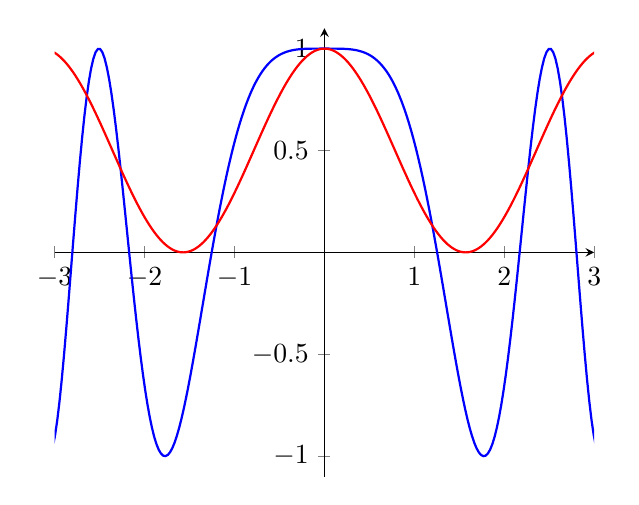
\begin{tikzpicture}
		\begin{axis}[xmin=-3,xmax=3,ymin=-1.1,ymax=1.1,axis x line=center,
		axis y line=center, restrict y to domain =-5:5]
		\addplot[thick,blue,samples=400] {cos(deg(x^2))};
		\addplot[thick,red,samples=400] {(cos(deg(x)))^2};
		\end{axis}
		\end{tikzpicture}
		\caption{Opgave~\ref{it:ssfunk1}}
		\label{fig:ssfunk1}
	\end{figure}
	
	\item Bestem $f\circ g$ og $g\circ f$ hvor $f(x)=\frac{1}{2}$ og $g(x)=4x^2+2x-1$.
	
	\item Lad $f\colon \{1,2,3\}\to \{a,b,c\}$ være givet ved $f(1)=b$, $ f(2)=a $, $ f(3)=c $. Bestem $g\colon \{a,b,c\}\to \{1,2,3\}$ så $g=f^{-1}$.
	
	\item Lad $f,g,h$ være funktioner defineret på $(0,\infty)$ givet ved
	\begin{align*}
	f(x)&=\sqrt{x},\\
	g(x)&=\frac{1}{1+x},\\
	h(x)&=\Big(\frac{1}{x}-1 \Big)^{2}.
	\end{align*}
	Bestem forskriften for følgende funktioner:
	\begin{enumerate}
		\item $f\circ g$,
		\item $g\circ f$,
		\item $f\circ h\circ g$,
		\item $g\circ h \circ f$,
		\item $ f\circ g \circ h $,
		\item $g\circ g$.
	\end{enumerate}
	
	
	\item Bestem den inverse funktion til $f\colon \R\setminus \{0\}\to \R\setminus\{0\}$ givet ved $f(x)=x^{-1}$. (Hint: Hvad er $f(f(x))$.)
	
	\item Vis at funktionerne $f\colon \R\setminus \{ \frac{1}{2}\}\to \R\setminus \{-\frac{1}{2} \}$ og $g\colon \R\setminus \{- \frac{1}{2}\} \to \R\setminus \{\frac{1}{2}\}$ givet ved
	\begin{align*}
	f(x)=\frac{x-1}{1-2x},&&g(x)=\frac{x+1}{1+2x},
	\end{align*}
	er inverse funktioner.
	
	\item Lad $f(x)=\cos((x-2)^2)$
	\begin{enumerate}
		\item Bestem funktioner $g$, $h$ så $f(x)=g(h(x))$.
		\item Bestem to andre funktioner $g_1$, $h_1$ så $f(x)=g_1(h_1(x))$
		\item Bestem tre funktioner $f_1,f_2,f_3$ så $f(x)=f_1(f_2(f_3(x)))$
	\end{enumerate}
	
	
	\item Lad funktionen $f(x)=e^{x^2}$ og bestem funktioner $g$ og $h$ så $f=g\circ h$.
	
	\item Lad $f\colon \R\to [-2,\infty[$ være givet ved $f(x)=(x-\sqrt{2})(x+\sqrt{2})$ og lad $g\colon [-2,\infty[\to [0,\infty[$ være givet ved $g(x)=\sqrt{x+2}$.
	\begin{enumerate}
		\item Bestem definitionsmængde, værdimængde og funktionsforskrift for $f\circ g$
		\item Er $g$ og $f$ inverse funktioner? (Hint: hvad er $(g\circ f)(-1)$?)
		\item Bestem en passende definitionsmængde $D$ så $f\colon D\to [-2,\infty[$ er invers til $g$.
	\end{enumerate}
	
		
	
	\item Betragt funktionerne $f\colon [0,\infty)\to [0,\infty)$ og $g\colon [0,\infty)\to[1,\infty)$ givet ved $f(x)=x^{3/2}$ og $g(x)=x^{2/3}+1$. 
	\begin{enumerate}
		\item Bestem det størst mulige domæne $D$ for funktionen $h\colon D\to \R$ givet ved $h(x)=x-1$ så sammensætningen $f \circ h$ er defineret.
		\item Vis at $g^{-1}=f\circ h$.
		\end{enumerate}
	
	%	
	
	
	
\end{enumerate}